\documentclass[letterpaper]{article}
\usepackage{aaai}
\usepackage{times}
\usepackage{helvet}
\usepackage{courier}
\usepackage{url}
\usepackage{graphicx}
\usepackage{grffile}
\usepackage{amsmath}
\usepackage{caption,subcaption}
\usepackage{algorithm,algorithmic}
\frenchspacing
\graphicspath{{./images/}}

\setlength{\pdfpagewidth}{8.5in}
\setlength{\pdfpageheight}{11in}

\pdfinfo{
/Title (Optimal Solvers for Minesweeper)
/Author (Nicholas Farn)
/Keywords (Minesweeper)
}

\title{Optimal Solvers for Minesweeper}
\author{Nicholas Farn\\ UCLA Department of Computer Science \\ nfarn@cs.ucla.edu}


\begin{document}
\maketitle

\begin{abstract}
Minesweeper is a single player computer game enjoyed by millions around the world.  Despite its simple rules and objective, Minesweeper is deceptively complex and actually belongs to a set of problems known as NP-Complete.  This paper approaches Minesweeper from the viewpoint of a constraint-satisfaction problem and goes over several solvers that achieve optimal or near optimal win-rates.
\end{abstract}

\section{Introduction}
Minesweeper is a single player game bundled with most Microsoft Windows operating systems.  It is played on an initially covered rectangular grid.  A set number of the spaces on the are secretly initialized to contain mines.  The goal of the game is to uncover all spaces on the grid that do not contain a mine, known as clearing the board.  If a mine is uncovered, the game ends immediately and the player loses.  If a space not containing a mine is uncovered, it displays the number of adjacent mines including diagonals.  Additionally, the first space uncovered in a game is always guaranteed to not be a mine.

For human players, the goal of Minesweeper is to clear a board in the least amount of time possible.  Accordingly, most strategy guides for Minesweeper focus on tactics to improve click speed with less concern on winning.  From the perspective of a computer scientist, this is uninteresting.  One could imagine a simple algorithm that may win only 0.01\% of the time but is able to play a single game in a fraction of a second.  Thus research is instead focused on optimal play for a game of Minesweeper.  However, a game of Minesweeper is not guaranteed to be deterministic, inevitably one is forced to guess.  Thus optimal play in a game of Minesweeper involves choosing the next space to uncover that has the least risk of losing given information currently provided by uncovered spaces.  Developing such algorithms that lead to optimal play is the crux of this paper.

\begin{figure}[t]
\centering
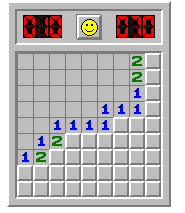
\includegraphics[width=0.5\columnwidth]{beginner}
\caption{A beginner level game of Minesweeper, played on a 9 $\times$ 9 grid with 10 mines.  The number of mines is displayed in the top left while the time taken is displayed on the right.  Uncovered spaces with no adjacent mines display an empty space rather than the number 0 by convention.  Minesweeper usually comes in 3 difficulties: beginner ($9 \times 9$ with 10 mines); intermediate ($16 \times 16$ with 40 mines); and expert ($16 \times 30$ with 99 mines).}
\label{fig:beginner_level}
\end{figure}

\section{Relevance}
% reference to Kaye, reference to Pederson
While Minesweeper may seem like a simple game, it actually belongs a class of problems known as NP-Complete.  As shown by Richard Kaye, determining whether a current game of Minesweeper is ``consistent'' is NP-Complete, where a consistent game of Minesweeper is a game where there exists an assignment of mines to spaces that can give rise to the current state.  This was further improved upon by Kasper Pederson, who showed that Minesweeper consistency is NP-Complete when the dimension of the board played upon is greater than 1.

However, in a normal game of Minesweeper it is safe to assume the board one is given is consistent.  Despite this, Minesweeper is still an interesting and relevant game to the field of Computer Science.  As also shown by Kaye, Minesweeper can be reduced into a SAT, a well known NP-Complete problem.  Additionally, the research in this paper seems to indicate finding optimal solutions to Minesweeper is at least as hard as solving an ALL-SAT problem, yet another well known NP-Complete problem.

\section{Prior Work}
Prior work on optimally solving Minesweeper seems to mostly be focused on approximating where to guess.  The earliest solver for Minesweeper appears to have been developed by John Ramsdell and implemented in freeware known as Programmer's Minesweeper (PGMS).  Unfortunately, PGMS appears to no longer be available online.  PGMS implemented two strategies to solve Minesweeper, single-point and equation strategy.  Both strategies are rather simplistic and perform well on beginner, but suffer terribly in performance on harder difficulties.

Minesweeper was first modeled as a constraint-satisfaction problem (CSP) by Chris Studholme.  Studholme also discovered that when given a set of equally risky moves, it is generally more advantageous to uncover spaces in a corner, then on an edge, and finally in the middle.  Other strategies include limited search, which models Minesweeper as a CSP as well, but approximates values in order to reduce the computational cost of Studholme's strategy.  Unfortunately, I discovered after development of the CSP set solver that it had been independently invented by Rapha\"el Collet who did not name the algorithm.  State of the art goes to Buffet et al, who also modeled Minesweeper as a CSP and created an ``optimistic heuristic'' to break ties.  Buffet et al named their solver Heuristic CSP (HCSP).

\section{Approaches}
A natural way of modeling Minesweeper is as a CSP.  Each space can be seen as a boolean variable, with it taking on a value of 1 if it contains a mine, or 0 if it is empty.  Each revealed space constrains the sum of its neighbors to be equal to the number of adjacent mines, i.e. the number revealed when uncovering a space.  Since the number of mines initialized are known beforehand, an additional constraint can be applied that requires the sum of all spaces to be equal to the number of initialized mines.  Variables can be named following standard matrix notation.  The state of a game of Minesweeper can then be seen as a set of known variable values, a set of covered variables, and a set of constraints.  It is important to note that the set of known variables is distinct from the set of covered variables as a variable could be covered but known to be a mine or safe.

\subsection{Simple Solvers}
\begin{figure}[t]
\centering
\begin{subfigure}[b]{0.45\columnwidth}
	\centering
	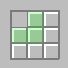
\includegraphics[width=\columnwidth]{simple constraint 0}
	\caption{\label{fig:simple_safe}}
\end{subfigure}
\begin{subfigure}[b]{0.45\columnwidth}
	\centering
	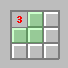
\includegraphics[width=\columnwidth]{simple constraint 1}
	\caption{\label{fig:simple_mine}}
\end{subfigure}
\caption{Example simple constraints.  In both \ref{fig:simple_safe} and (\ref{fig:simple_mine}), the top-left space, $x_{1,1}$, placing a constraint on its highlighted neighbors.  For (\ref{fig:simple_safe}), the constraint is $x_{1,2} + x_{2,1} + x_{2,2} = 0$, which results in all highlighted spaces being 0 or safe.  For (\ref{fig:simple_mine}), the constraint is $x_{1,2} + x_{2,1} + x_{2,2} = 3$, which requires all highlighted spaces to be 1 or mines.}
\end{figure}

Using this framework, it is easy to solve some constraints just by viewing the value the variables are constrained to sum to.  If all the variables in a constraint are constrained to sum to 0, then every variable must be 0 and can be safely uncovered.  Conversely, if there are $n$ variables in a constraint, and the variables are constrained to sum to $n$, then every variable must be 1 and can be recorded as a known mine.  Constraints that can be used to solve variables in such a way are referred to as simple constraints.  Safe spaces and known mines can be recorded and used to simplify other constraints further.

Solving constraints and propagating this information to other constraints is the crux of single-point strategy.  When forced to guess, single-point strategy chooses an unknown space to uncover with a uniform probability.  This strategy can be improved upon further by noting that the set of variables that appear in a particular constraint may be a subset of variables that appear in another constraint.  
Newly simplified constraints can then be used to simplify or solve more constraints.  For example, given the constraints (\ref{eq:simple_constraints}), the second constraint can be simplified using the first constraint with the use of linear algebra.  The second constraint then becomes $x_{1,3} + x_{2,3} = 0$, a simple constraint.

\begin{equation}\label{eq:simple_constraints}
\begin{aligned}
x_{1,3} + x_{2,3} + x_{2,1} + x_{2,2} &= 1\\
x_{2,1} + x_{2,2} &= 1
\end{aligned}
\end{equation}

Simplifying and solving constraints in such a manner is equation strategy.  Equation strategy simplifies and solves as many constraints as it can and uncovers as many spaces as it can before it is forced to guess.  Like single-point strategy, when it is forced to guess, equation strategy simply chooses an unknown space to uncover with uniform probability.  All subsequent algorithms are essentially the same as equation strategy as they simplify and solve constraints in exactly the same way.  The only difference is how subsequent algorithms determine which space to uncover when forced to guess.  The pseudocode for a general solver can be seen at algorithm (\ref{alg:general_solver}).

\begin{algorithm}[t]
\caption{General Minesweeper Solver}
\label{alg:general_solver}
\begin{algorithmic}[1]
\STATE initialize set of covered spaces $C$ to contain all spaces
\STATE initialize set of safe spaces $S$ to empty
\STATE initialize set of known mines $M$ to empty
\WHILE{$C \neq \emptyset$}
	\IF{$C \cup S \neq \emptyset$}
		\STATE assign space in $C \cup S$ to uncover
	\ELSE
		\STATE use guessing algorithm
	\ENDIF
	\IF{uncovered space is not a mine}
		\STATE remove space from $C$
		\STATE add space to $S$
		\STATE add new constraint from space
		\STATE simplify constraint using $S$ and $M$
		\IF{new constraint is now simple}
			\STATE add variables to $S$ or $M$
		\ENDIF
		\STATE simplify remaining constraints
	\ENDIF
\ENDWHILE
\end{algorithmic}
\end{algorithm}

Without taking into account the time complexity of the guessing algorithm, the time complexity of algorithm (\ref{alg:general_solver}) is $O(n^2)$ where $n$ is the number of variables.  This is because there can be at most $n+1$ constraints to consider if there are $n$ variables.

\subsection{CSP Solver}
The basic CSP algorithm chooses where to guess by uncovering an unknown space with the lowest probability of being a mine.  The probability of a space being a mine can be calculated by taking the average assigned value to a space over all unique assignments that satisfy the currently revealed constraints.  The probability calculated is the exact probability as there is a uniform probability of any of the unique assignments occurring since the initial probability of a space being a mine is uniform at the beginning of the game.  However, finding all unique valid assignments boils down into solving an ALL-SAT problem.  This can be done through the use of a backtracking depth first search.  However, this is expensive as the worst-case time complexity of such an algorithm is $O(2^n)$ given $n$ variables.  The performance can be improved through the use of variable ordering and backjumping.  These can both be calculated when checking constraints to see if an assignment is valid and add no extra complexity when generating a node.  Variable ordering by itself significantly improves performance.

Performance can be even furthered improved by separating unknown variables into disjoint sets.  A single set would consist only of variables that only appear in a constraint with other variables in the set for all constraints.  For example suppose there exists three constraints at (\ref{eq:disjoint_sets}), none of the variables that appear in the first two constraints appear in the third.  Therefore two sets can be formed, $\{x_{1,1}, x_{1,2}, x_{1,3}\}$ and $\{x_{2,1}, x_{2,2}, x_{2,3}\}$.

\begin{equation}\label{eq:disjoint_sets}
\begin{aligned}
x_{1,1} + x_{1,2}& &= 1\\
x_{1,2} &+ x_{1,3} &= 1\\
x_{2,1} + x_{2,2} &+ x_{2,3} &= 2
\end{aligned}
\end{equation}

In terms of a constraint graph, variables in a set would only be able to travel to other variables within the set where edges form between variables that are in a constraint together.  Then the backtracking algorithm can be performed on each set separately, since variables in a single set cannot affect how constrained variables outside of their set are.  This greatly improves performance early in the game since revealed spaces are more likely to be far apart and resulting in little to no overlap.

However, despite these improvements, the basic CSP algorithm is only able to solve some beginner level games.  This is due to the fact that on average it only needs to make approximately 1.1 guesses a game.  Thus for a good number of games it does not even need to make a guess, or is given a single constraint that does not require a backtracking algorithm to solve.

\subsection{CSP Set Solver}
The basic CSP algorithm can be vastly improved by forming a single variable equal to the sum of a set of variables.  The set of variables chosen to be summed into a single variable always appear together across all constraints.  In other words, they are all constrained by the same set of constraints and thus will have the same probability of being a mine.  For example, take the following two constraints at (\ref{eq:set_variables}).  Variables $x_{1,2}$ and $x_{1,3}$ appear together in both the first two constraints, thus they can be summed into a single ``set'' variable, $s = x_{1,2} + x_{1,3}$.

\begin{equation}\label{eq:set_variables}
\begin{aligned}
x_{1,1} + x_{1,2} &+ x_{1,3}&&&= 1\\
x_{1,2} &+ x_{1,3} &+ x_{2,1}&&= 2\\
&&x_{2,2} &+ x_{2,3} &= 1
\end{aligned}
\end{equation}

Constraints can then be rewritten in terms of set variables reducing the number of variables needed to be considered when performing a backtracking DFS.  The probability of a space containing a mine can then be computed by dividing the expected assigned value to a set variable by the number of variables summed in the set variable.  However, these new set variables are no longer boolean variables and can take on a potential of integer values from 0 to the number of variables summed in a single set variable.  

Despite the increased branching factor of the search, the reduction in search depth always makes forming set variables worth it.  Suppose $N$ nodes are generated in a run of a backtracking algorithm.  Let two variables be joined into a single set variable.  In the best case, all possible combinations of values can be assigned to the two removed variables.  Thus removing them results in a multiplicative reduction of 4 at best.  Since all assignments are valid between the two variables, the set variable can be assigned 0, 1, or 2 as values, resulting in a multiplicative increase of 3.  Overall this leads to an improvement of $\frac34 N$ nodes generated in the best case.  In general, forming a set variable which is the sum of $m$ variables results in a multiplicative reduction of at most $\frac{1}{2^m}\min(m+1,k)$ where $k$ is the number of remaining unknown mines.  In the worst case, no set variables can be formed, or the set variable is constrained to equal only 0 resulting in the exact same number of nodes generated.  Therefore the worst-case time complexity is still $O(2^n)$ where $n$ is the number of variables.

In practice, although the maximum improvement is rarely achieved, set variables lead to vast improvements in performance.  Just like disjoint set, set variables are almost guaranteed to form early and even into mid-game.  By end-game, there are few enough variables to consider that an ordinary backtracking DFS does fine although small set variables do form.  The CSP set solver was able to solve all three difficulties of Minesweeper in reasonable time where the basic CSP solver was barely able to solve the first.  The win rate for both solvers are exactly the same since the exact same probabilities are computed by both guessing algorithms.

\subsection{Globally Optimal Solver}
Unfortunately, neither CSP solver returns globally optimal guesses.  A good way to see why this is so is to consider what happens when there are multiple spaces of minimum probability of being a mine.  Suppose we have the initial state in figure (\ref{fig:initial_state}).  There is only a single constraint which gives every space a uniform probability of $\frac25$ of being a mine.  Suppose the space chosen does not contain a mine, what is the information gained?  Choosing the space in figure (\ref{fig:suboptimal_state}) will always reveal a 2 leading to a 50-50 guess.  However, if a corner is chosen instead like in figure (\ref{fig:optimal_state}), there is a $\frac13$ probability of the space revealing a 0 or 2 which would lead to a win without needing to guess.  Thus revealing the space in figure (\ref{fig:suboptimal_state}) will lead to a higher probability of losing in the long run.  Therefore an optimal solver for Minesweeper will not choose a space with the minimum probability of containing a mine, but the space that leads to the lowest probability of losing in the long run.  This also implies that the most optimal move will not necessarily also be a space with the lowest probability of being a mine.

\begin{figure}[t]
\centering
\begin{subfigure}[b]{0.3\columnwidth}
	\centering
	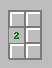
\includegraphics[width=\columnwidth]{tie breaker 1}
	\caption{\label{fig:initial_state}}
\end{subfigure}
\begin{subfigure}[b]{0.3\columnwidth}
	\centering
	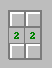
\includegraphics[width=\columnwidth]{tie breaker 2}
	\caption{\label{fig:suboptimal_state}}
\end{subfigure}
\begin{subfigure}[b]{0.3\columnwidth}
	\centering
	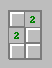
\includegraphics[width=\columnwidth]{tie breaker 3}
	\caption{\label{fig:optimal_state}}
\end{subfigure}
\label{fig:tie_breaker}
\caption{The initial state in (\ref{fig:initial_state}) gives a uniform probability of $\frac25$ of revealing a mine for all spaces.  If the space revealed in (\ref{fig:suboptimal_state}) is not a mine it will be a two, resulting in a total probability of $\frac{7}{10}$ of losing by revealing that space.  However, if one reveals the space in (\ref{fig:optimal_state}) and it is not a mine, one is given a guaranteed win $\frac13$ of the time and a 50-50 win the remaining $\frac23$.  This leads to a total probability of $\frac35$ of losing.}
\end{figure}

The pseudocode for an algorithm that is able to calculate globally optimal guesses can be viewed at algorithm (\ref{alg:optimal_guesser}).  Essentially, the algorithm calculates the probability of losing by revealing a given space by considering every potential future game given the currently revealed constraints.  Potential games can be computed through the use of the backtracking DFS algorithm used in the CSP solver.  However, the CSP set solver cannot be used since it calculates probabilities by eliminating variables of the same probability, a feature no longer nearly as present.  In this case the exact assignment of values to variables is needed to simulate potential games and how well they play out in favor for the solver.  However, while simulating a potential game, if the solver is forced to guess in the potential game it must determine where it will guess which requires a recursive call to the already expensive guessing algorithm.

\begin{algorithm}[t]
\caption{Optimal Guesser}
\label{alg:optimal_guesser}
\begin{algorithmic}[1]
\STATE initialize running average 
\FOR{unique valid game state}
	\FOR{covered space}
		\STATE uncover space
		\IF{space is mine}
			\STATE win probability is 0
		\ELSE
			\STATE simplify and solve constraints
			\IF{game is won}
				\STATE win probability is 1
			\ELSE
				\STATE recursively compute win probability of remaining spaces
				\STATE win probability is maximum of returned probabilities
			\ENDIF
		\ENDIF
	\ENDFOR
	\STATE record win probability of space in running average
\ENDFOR
\RETURN win probabilities of all covered spaces
\end{algorithmic}
\end{algorithm}

Worst of all, such an algorithm barely performs better the CSP set solver.  One is trading large amounts of performance in return for small improvements in the win rate of 1-2\%.  While this solver can certainly be improved to prevent fewer recursive calls, it still has to consider every possible game given the current constraints.  The reason behind this is simple, suppose there is a globally optimal solver that does not need to consider every possible game state.  Then even on simple boards, if the game state it does not consider is the actual game state then it will return suboptimal results.  Therefore at best any globally optimal solver that considers probabilities has a lower bound on the time-complexity of $O(2^n)$.

For algorithm (\ref{alg:optimal_guesser}), given $n$ variables, its performance in the best case is $O(n^32^n)$ per guess as it must generate $O(2^n)$ states and perform algorithm (\ref{alg:general_solver}) assuming the generated state on every covered space, an $O(n^3)$ operation.  This is assuming no guesses are needed and thus no recursive calls.  The worst-case time complexity is $O(\Pi_1^n n^32^n)$.

\subsection{Tie-Breaking Solvers}
A variation of the CSP set solver was implemented to break ties when there are multiple spaces of minimum probability of being a mine.  The solver breaks ties by choosing spaces with the least number of adjacent squares whose values are currently unknown.  The logic behind this is based on prior work by Studholme, who demonstrated it is most advantageous to choose corners, then edges, then middles when a guess is needed early game.  The main reasoning by Studholme was that corners had far fewer adjacent spaces and had a greater likelihood of revealing a zero for a constraint leading to more information gain.  The natural extrapolation would then be to choose spaces with the least number of unknown adjacent spaces as they are most likely constrain their unknown neighbors to zero given a relatively similar probability.

This tie-breaking solver performs as well as state of the art and does generally better than a uniform guess between minimum probabilities.  It was largely developed in order to compare its performance against the globally optimal solver.  The globally optimal solver may also encounter tied probabilities.  However, since these probabilities are globally optimal, there is no benefit in breaking them.

\section{Experimental Results}
In order to characterize the performance of the various solvers, I ran trials on all 3 difficulties for CSP set solver and tie-breaking.  These results are also compared to other solvers and can be viewed in table (\ref{tb:win_percent}).  The global solver was compared to a simple tie-breaking solver by running both on a small, 3x3 board for numerous trials.  These results can be viewed in table (\ref{tb:global_percent}).  Larger boards were attempted, but a sufficient number of trials was not reached in order to draw conclusive results.  Furthermore, a comparison of nodes generated over the course of a game was done between the basic CSP solver and CSP set solver in order to compare the average improvement between the two, table (\ref{tb:nodes}).  Generally, the mine count for smaller board was chosen to have a similar density as expert difficulty in order to encourage more guesses per game.%

\begin{table}[h]
\centering
\resizebox{\columnwidth}{!}{
\begin{tabular}{|c|c|c|c|c|c|c|}
\hline
& Equation & Limited Search & CSP set solver & Tie-breaking & HCSP \\
\hline
Beginner & 71\% & 92\% & 89\% & 90\% & 89\% \\
Intermediate & 36\% & 64\% & 74\% & 76\% & 74\% \\
Expert & 26\% & 17\% & 31\% & 34\% & 38\% \\
\hline
\end{tabular}
}
\caption{Win percentage of various solvers over standard difficulty levels for at least 1000 games.}
\label{tb:win_percent}
\end{table}

\begin{table}[h]
\centering
\resizebox{\columnwidth}{!}{
\begin{tabular}{|c|c|c|c|}
\hline
& CSP set solver & tie-breaking & Globally optimal\\
\hline
$3\times3$ with 2 mines & 77\% & 80\% & 82\% \\
\hline
\end{tabular}
}
\caption{Comparison of win rate over for at least 500 games.}
\label{tb:global_percent}
\end{table}

\begin{table}[h]
\centering
\resizebox{0.8\columnwidth}{!}{
\begin{tabular}{|c|c|c|}
\hline
& CSP solver & CSP set solver \\
\hline
$4 \times 4$ with 3 mines & 56.22 & 7.38 \\
$5 \times 5$ with 5 mines & 3,230.18 & 31.56 \\
$6 \times 6$ with 7 mines & 607,889.64 & 84.44 \\
\hline
\end{tabular}
}
\caption{Comparison of nodes generated for a variety of board sizes.}
\label{tb:nodes}
\end{table}

\section{Conclusion}
To my knowledge there has been no previous work on designing and characterizing a globally optimal solver for Minesweeper.  However, as the experimental results indicate, a globally optimal solver barely performs better than the tie-breaking CSP set solver.  However, the global algorithm could potentially be significantly improved in future work as it exhibits many symmetries when computing probabilities.  Overall, it is interesting to see that the vast majority of moves made in Minesweeper are not guesses.  Even on the hardest difficulty, the tie-breaking CSP set solver would make approximately 7.4 guesses a game.  This drops drastically for easier difficulties with intermediate at 2.5 guesses and beginner around 1.1.  It was also surprising how much of an improvement the CSP set solver made over a basic CSP solver as it made possible playing all three difficulties with expert usually taking approximately 3 seconds.  Thus is in comparison to the CSP solver taking most of a day on some beginner level games.

\bibliography{minesweeper}
\bibliographystyle{aaai}
\nocite{*}
\end{document}